%\subsection{Images créées}
\SbSSCT{Images créées}{Own small pictures}

\begin{center}
\RRR{14-19 }  \RRR{18 }
\end{center}

\bigskip

\tikzset{dfr/.pic={\filldraw[blue] (-2pt,0) rectangle (0,5pt) ; \filldraw[fill=white] (0,0) rectangle (2pt,5pt); \filldraw[fill=red] (2pt,0) rectangle (4pt,5pt); }}

%création

\begin{tabular}{|c|c|}\hline 
\textbf{Création}  & \textbf{ Utilisation} \\ \hline 
\parbox{10cm}{\BS{tikzset}\AC{{\color{red}{dfr/.pic}}=\AC{\BS{filldraw}[blue] (-2pt,0) rectangle (0,5pt) ; \\ \BS{filldraw[fill=white] (0,0) rectangle (2pt,5pt);\\ \BS{filldraw}[fill=red] (2pt,0) rectangle (4pt,5pt); }}}}
&
\parbox{3cm}{\BS{tikz} \BSS{pic} \AC{dfr}; \\
\tikz \pic {dfr};} 
\\ \hline 
\end{tabular} 


\bigskip
%placement à une position

\begin{tabular}{|c|c|c|} \hline 
\multicolumn{2}{|c|}{\textbf{\TFRGB{placement à une position}{Positioning }}}
\\ \hline 
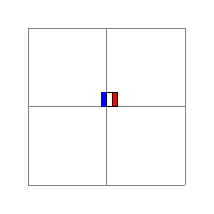
\begin{tikzpicture}
\draw[help lines] (0,0) grid (2,2) ; 
\pic at (1,1) [pic type = dfr]; 
  \end{tikzpicture} 
&  
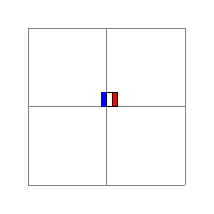
\begin{tikzpicture}
\draw[help lines] (0,0) grid (2,2) ; 
\pic at (1,1) {dfr}; 
\end{tikzpicture}
\\ \hline 
\BSS{pic} at (1,1) [\RDD{pic type} = dfr]; & 
\BSS{pic} at (1,1) \AC{dfr};  
\\ \hline   
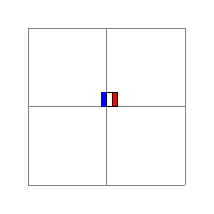
\begin{tikzpicture}
\draw[help lines] (0,0) grid (2,2) ; 
\path (1,1) pic [pic type = dfr];
\end{tikzpicture} 
&  
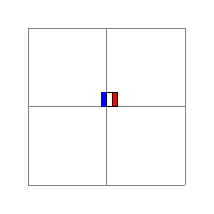
\begin{tikzpicture}
\draw[help lines] (0,0) grid (2,2) ; 
\path (1,1) pic {dfr};
\end{tikzpicture} 
\\ \hline 
\BS{path} (1,1) \RDD{pic} [\RDD{pic type}= dfr]; &
\BS{path} (1,1) \RDD{pic} \AC{dfr};
\\ \hline
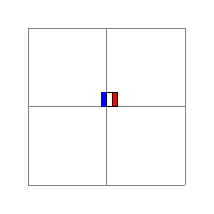
\begin{tikzpicture}
\draw[help lines] (0,0) grid (2,2) ; 
\pic [at={(1,1)},pic type = dfr];
\end{tikzpicture}
& 
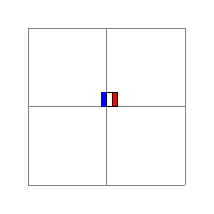
\begin{tikzpicture}
\draw[help lines] (0,0) grid (2,2) ; 
\pic [at={(1,1)}] {dfr};
\end{tikzpicture}  
\\ \hline   
 \BSS{pic} [at=\AC{(1,1)}] [\RDD{pic type}= dfr]; &
 \BSS{pic} [at=\AC{(1,1)}] \AC{dfr}; 
\\ \hline
\end{tabular}

\bigskip

\begin{tabular}{|c|c|c|} \hline 
\multicolumn{3}{|c|}{\BS{pic}[scale=3] at (1,1) \AC{dfr}; }
\\ \hline 
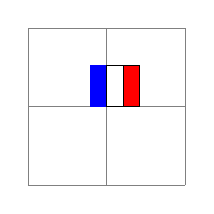
\begin{tikzpicture}
\draw[help lines] (0,0) grid (2,2) ; 
\pic[scale=3] at (1,1) {dfr}; 
  \end{tikzpicture}
&  
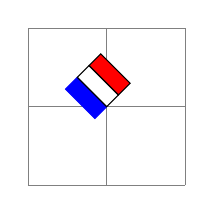
\begin{tikzpicture}
\draw[help lines] (0,0) grid (2,2) ; 
\pic[scale=3,rotate=45] at (1,1) {dfr}; 
  \end{tikzpicture}
&  
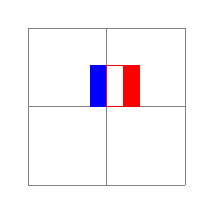
\begin{tikzpicture}
\draw[help lines] (0,0) grid (2,2) ; 
\pic[scale=3,red] at (1,1) {dfr}; 
  \end{tikzpicture} 
\\ \hline 
[{\color{red}scale}=3] & [scale=3,{\color{red}rotate}=45] & [scale=3,{\color{red}red}] \\ 
\hline 
\end{tabular} 

\bigskip

\begin{tabular}{|c|c|} \hline  
\parbox{8cm}{\BS{tikz} [scale=4] {
\BS{pic} at (0,0) \AC{dfr}; \\
\BS{pic} at (.5,0) [\RDD{transform shape}] \AC{dfr};
}}
&  
\tikz [scale=4] {
\pic at (0,0) {dfr};
\pic at (.5,0) [transform shape] {dfr};
}
\\ \hline  
\end{tabular}  

\bigskip

\begin{tabular}{|c|} \hline
\textbf{\TFRGB{Placement sur un chemin}{On a path}}
\\ \hline    
\BS{tikz} \BS{draw}
(0,0) to [out=10,in=170]
pic [{\color{red} near start}] \AC{dfr}
pic \AC{dfr} \\
pic [{\color{red} sloped, near end}] \AC{dfr} (10,0);
\\ \hline  
\tikz \draw
(0,0) to [out=10,in=170]
pic [near start] {dfr}
pic {dfr}
pic [sloped, near end] {dfr} (10,0);
\\ \hline  
\BS{draw} (0,0) to [out=10,in=170] pic [pos=.3]  \\
\AC{\RDD{code}=\AC{\BS{draw} circle [radius=3mm];}} (10,0)  ;
\\ \hline  
\tikz \draw (0,0) to [out=10,in=170] 
pic [pos=.3] {code={\draw circle [radius=3mm];}} (10,0)  ;
\\ \hline 
\end{tabular} 


\tikzset{ my pic/.pic = {
\path [pic actions] (0,0) circle[radius=3mm];
\draw (-3mm,-3mm) rectangle (3mm,3mm);} }

\bigskip
\begin{tabular}{|c|c|c|c|c|} \hline
 \multicolumn{5}{|l|}{ Définition :} \\
 \multicolumn{5}{|l|}{ \BSS{tikzset}\{ my pic/.pic = \{ }\\
 \multicolumn{5}{|l|}{  \BS{path} [\RDD{pic actions}] (0,0) circle[radius=3mm];} \\
\multicolumn{5}{|l|}{ \BS{draw} (-3mm,-3mm) rectangle (3mm,3mm); \}  \} }
 \\ \hline 
 \multicolumn{5}{|c|}{ Utilisation : \hspace{2cm}\BS{pic} [red] \AC{my pic} }
 \\ \hline 
\tikz \pic [red] {my pic}; 
&
\tikz \pic [draw] {my pic};
&  
\tikz \pic [draw=red] {my pic};
&  
\tikz \pic [draw, shading=ball] {my pic};
&  
\tikz \pic [fill=red!50] {my pic};
\\ \hline  
[red] & [draw]  &  [draw=red]  &  [draw, shading=ball]  &   [fill=red!50] 
\\ \hline 
\end{tabular} 

\bigskip

\begin{tabular}{|c|} \hline  
\BS{tikz} \BS{pic} foreach \BS{x} in \AC{1,1.5,...,10} at (\BS{x},0) \AC{dfr};
\\ \hline  
\tikz \pic foreach \x in {1,1.5,...,10} at (\x,0) {dfr};
\\ \hline 
\end{tabular} 

\bigskip

\begin{tabular}{|c|c|} \hline 
 \multicolumn{2}{|l|}{ \BS{fill} [green]
 (0,0) - - (1,0)pic [\RDD{behind path},scale=3] \AC{dfr} -- (1,1) -- (0,1) -- cycle ;} 
 \\ \hline 
 
\tikz \fill [green]
(0,0) -- (1,0)pic [behind path,scale=3] {dfr} -- (1,1) -- (0,1) -- cycle ;
&  
\tikz \fill [green]
(0,0) -- (1,0)pic [scale=3] {dfr} -- (1,1) -- (0,1) -- cycle ;
\\ \hline 
[\RDD{behind path},scale=3] & [scale=3] \\ 
\hline 
\end{tabular} 

\bigskip

\begin{tabular}{|c|c|} \hline 
\parbox{10cm}{ 
\BSS{tikzset}\AC{
pics/{\color{purple}mon cercle}/.style = \AC{
\RDD{background code} = \AC{ \BS{fill} circle [radius={\color{blue}\#1}]; }
}
}\\
\BS{tikz} [fill=green]
\BS{draw}[line width=3pt]  (0,0) pic \AC{{\color{purple}mon cercle}={\color{blue}2mm}} - - (1,1) pic \AC{{\color{purple}mon cercle}={\color{blue}5mm}};}
&
\tikzset{
pics/mon cercle/.style = {
background code = { \fill circle [radius=#1]; }
}
}
\tikz[baseline=.5cm,fill=green]
\draw[line width=3pt]  (0,0) pic {mon cercle=2mm} -- (1,1) pic {mon cercle=5mm};
\\ \hline
\parbox{10cm}{ 
\BSS{tikzset}\AC{
pics/{\color{purple}mon cercle}/.style = \AC{
\RDD{foreground  code} = \AC{ \BS{fill} circle [radius={\color{blue}\#1}]; }
}
}\\
\BS{tikz} [fill=green]
\BS{draw}[line width=3pt]  (0,0) pic \AC{{\color{purple}mon cercle}={\color{blue}2mm}} - - (1,1) pic \AC{{\color{purple}mon cercle}={\color{blue}5mm}};} 
&
\tikzset{
pics/mon cercle/.style = {
foreground code = { \fill circle [radius=#1]; }
}
}
\tikz[baseline=.5cm,fill=green]
\draw[line width=3pt]  (0,0) pic {mon cercle=2mm} -- (1,1) pic {mon cercle=5mm};
\\ \hline
\end{tabular} 

\bigskip

\begin{tabular}{|c|c|}\hline 
\parbox{11cm}{ 
 \BS{fill} [green](-1,0) - - (1,0) \\ 
pic [pics/\RDD{background code}=\AC{\BS{fill}[blue] (0.5,0.5) circle (1cm );}\\
, pics/code={\BS{fill}[red] (-1,-.5) rectangle (0.5,0.5);} ]\\ \AC{} - - (1,2) - - (-1,2) - - cycle ;}
&  
\tikz[baseline=1cm] 
\fill [green] (-1,0) -- (1,0)  
pic [pics/background code={\fill[blue] (.5,.5) circle (1cm );}
, pics/code={\fill[red] (-1,-.5) rectangle (.5,.5);} ]  {} -- (1,2) -- (-1,2) -- cycle ;
\\ \hline
  
\parbox{11cm}{ 
 \BS{fill} [green] (-1,0) - - (1,0) \\ 
 pic [pics/\RDD{foreground code}={\BS{fill}[blue] (0.5,0.5) circle (1cm );}\\
,pics/code=\AC{\BS{fill}[red] (-1,-.5) rectangle (0.5,0.5);} ]\\ \AC{} - - (1,2) - - (-1,2) - - cycle ;}
&  
\tikz[baseline=1cm]  \fill [green]
(-1,0) -- (1,0)pic [pics/foreground code={\fill[blue] (.5,.5)circle (1cm );},pics/code={\fill[red] (-1,-.5) rectangle (.5,.5);} ] {} -- (1,2) -- (-1,2) -- cycle ;
\\ \hline  
\parbox{11cm}{ 
 \BS{fill} [green](-1,0) - - (1,0) \\ 
pic [pics/\RDD{background code}=\AC{\BS{fill}[blue] (0.5 , 0.5) circle (1cm );}\\
,pics/code=\AC{\BS{fill}[red] (-1 , -0.5) rectangle (0.5 , 0.5);},\RDD{behind path} ]\\ 
\AC{} - - (1,2) - - (-1,2) - - cycle ;}
&  
\tikz[baseline=1cm]  
\fill [green](-1,0) -- (1,0) 
pic [pics/background  code={\fill[blue] (.5,.5) circle (1cm );} , pics/code={\fill[red] (-1,-.5) rectangle (.5,.5);},behind path ] {} -- (1,2) -- (-1,2) -- cycle ;
\\ \hline 
 
\parbox{11cm}{ 
 \BS{fill} [green]
(-1,0) - - (1,0) \\
 pic [pics/\RDD{foreground code}=\AC{\BS{fill}[blue] (0.5 , 0.5) circle (1cm );}\\
, pics/code=\AC{\BS{fill}[red] (-1,-.5) rectangle (0.5 , 0.5);},\RDD{behind path} ]\\ 
\AC{} - - (1,2) - - (-1,2) - - cycle ;
}
&  
\tikz[baseline=1cm]  
\fill [green](-1,0) -- (1,0)
pic [pics/foreground code={\fill[blue] (.5,.5)circle (1cm );},pics/code={\fill[red] (-1,-.5) rectangle (.5,.5);},behind path ] 
{} -- (1,2) -- (-1,2) -- cycle ;
\\ \hline 

\end{tabular} 
   